\chapter{Background} \label{chap:Background}

In this chapter, we describe the research which led to the current project. In Section \ref{sec:MapReduce}, we provide an overview of the MapReduce framework and subsequently the Hadoop MapReduce implementation \cite{HadoopWeb}.  

Furthermore, in Section \ref{sec: DataCentreArch} we describe the current state-of-the art in data centre architecture design and focus on  \textit{fat-tree} \cite{al2008scalable} data centre topology in \ref{subsec:Fat-Tree Topology}, which is used in our experiment as the network topology because of its ability to alleviate inter-node communication bandwidth bottlenecks in large-scale clusters. 

Finally, in Section \ref{sec:Flow Scheduling in Data Centres} we describe the current state-of-the-art \textit{flow scheduling} mechanisms for in data centre networks, namely Equal Cost Multi-Path Routing (ECMP \cite{hopps2000analysis}) and Global First-Fit \cite{al2010hedera}, implementations of which are used in our experiment to compare against proactive measures of flow scheduling.   

\section{MapReduce} \label{sec:MapReduce}

\begin{figure}[!ht]
\centerline{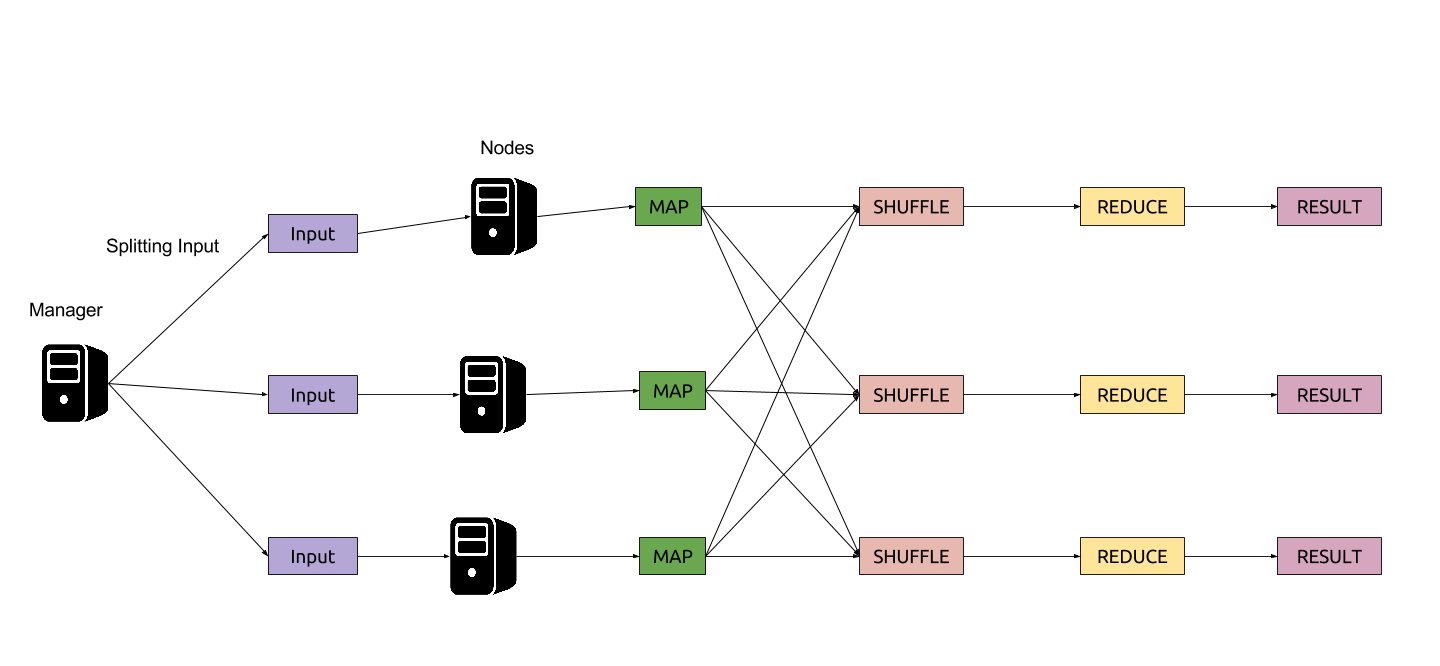
\includegraphics[scale=0.30]{GeneralMapReduce.png}}
\caption{High level overview of the MapReduce Framework.}
\label{fig:MROverview}
\end{figure}

MapReduce was introduced by Dean \textit{et al.} \cite{dean2008mapreduce} as a programming abstraction, which enables distributed cluster computing with commodity servers and is highly fault tolerant and reliable. MapReduce is one of the most frequently used framework for big data processing \cite{barroso2013datacenter} and we chose it for our project due to its ubiquity and popularity. It broadly consists of 3 phases, namely the \textit{map}, \textit{shuffle} and \textit{reduce} phases as illustrated in Figure \ref{fig:MROverview}. 
  
MapReduce is a computational model based on \textit{key-value} pairs. The \textit{Map} function produces a set of intermediate \textit{key-value} pairs for a given input \cite{dean2008mapreduce}. Subsequently, the intermediate data is grouped according to its keys in the \textit{shuffle} phase. Finally, in the \textit{reduce} phase, all values for a given key are combined to produce the final result. The data used for MapReduce jobs is usually stored in a distributed file system (DFS), which takes care of fault tolerance by replicating the data across the cluster. Examples of such data stores include GFS \cite{ghemawat2003google} and HDFS \cite{borthakur2008hdfs}.

\subsection{High Level Execution Overview} \label{subsec:MROverview}

The input data set of a MapReduce job is first partitioned into \textbf{M} pieces, which are processed in parallel by different machines \cite{dean2008mapreduce}. The Reduce function is invoked by partitioning the intermediate key set of the data into a set of \textbf{R} pieces, which is distributed across the entire cluster for computation. 

MapReduce computation proceeds in the following steps

\begin{itemize}
\item The input file is first split into \textbf{M} pieces while MapReduce starts up on the entire cluster of machines.
\item One of the machines in the cluster is designated as the \textit{master} node, while all the other nodes in the network are \textit{worker} nodes which are assigned jobs by the \textit{master} node. The master assigns a map task or a reduce task to each one of the idle worker nodes in the network from a total of \textbf{M} map tasks and \textbf{R} reduce tasks.
\item The corresponding partitioned input is read by the worker which is assigned a map task, it parses the input and emits key-value pairs and passes each of those to the map function. Intermediate key-value pairs emitted by the map function are buffered in memory.
\item The buffered pairs are written into persistent memory store of the worker nodes on a periodic basis and are partitioned into \textbf{R} pairs. Memory locations of these key-value pairs are sent to the master node so that they can be forwarded to the reduce worker nodes \cite{dean2008mapreduce}.
\item On notification about these locations, the reduce worker reads the buffered data from the persistent memory store of the map workers via RPC calls \cite{dean2008mapreduce}. Subsequently, it sorts the intermediate keys of the data by grouping the same keys together, this is also called the shuffling phase. 
\item  The sorted intermediate data is iterated upon by the reduce worker nodes and for each unique key encountered, it passes the corresponding key-value pairs to the reduce function. 
\end{itemize}

After all the above steps culminate, the output consists of \textbf{R} output files. These files may or may not be merged into a single output file, depending on the MapReduce implementation. 

\subsection{Hadoop Overview} \label{subsec:HadoopOverview}

Hadoop is one of the most frequently used open source MapReduce implementations. We choose Hadoop as the MapReduce implementation of choice for this project due to it being open source and its widespread usage for Big Data analysis. It broadly consists of \textit{two} main components   
\begin{itemize}
\item Hadoop MapReduce - Open-source implementation of the MapReduce computation model.
\item HDFS (Hadoop Distributed File System) - A resilient, fault tolerant and distributed file system that provides high throughput access to application data and is designed to be used with commodity hardware \cite{borthakur2008hdfs}.
\end{itemize}
\begin{figure}[!ht]
\centerline{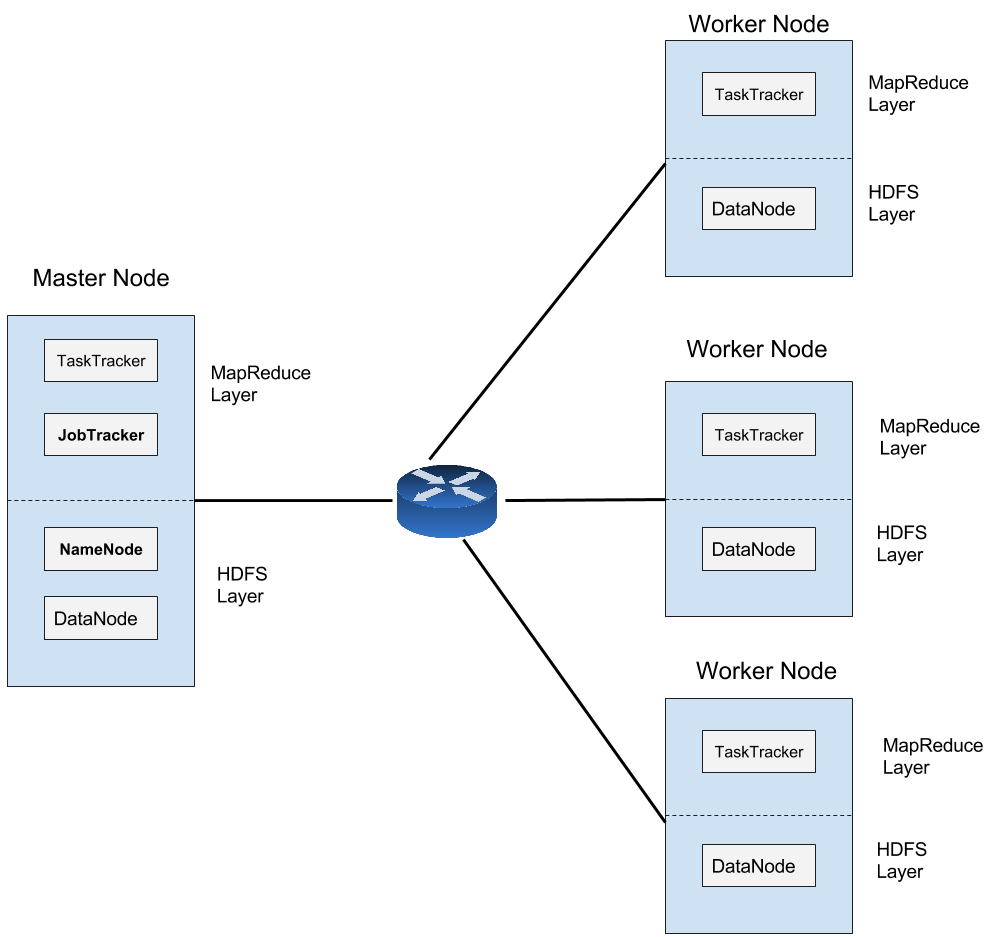
\includegraphics[scale=0.35]{HadoopArchitecture.png}}
\caption{Basic Hadoop Architecture with the master node housing the JobTracker and the NameNode functionalities of Hadoop, while the worker (slave) nodes housing the TaskTracker and DataNode functionalities of Hadoop.}
\label{fig:HadoopArchitecture}
\end{figure}

Similar to the Google MapReduce model \cite{dean2008mapreduce} outlined in Section \ref{sec:MapReduce}, HDFS too has a master-slave architecture \cite{borthakur2008hdfs}. As illustrated in Figure \ref{fig:HadoopArchitecture} a Hadoop cluster consists of the following
\begin{itemize}
	\item HDFS layer consists of two types of nodes responsible for managing the Distributed file system 
    	 \begin{itemize}
		  \item \textbf{NameNode} - The entire Hadoop cluster contains one \textit{NameNode} which serves as the master server, managing the file system access of worker nodes and the file system name space. It also instructs the \textit{DataNodes} (slaves) in the cluster to create, delete and replicate data blocks.
		  \item \textbf{DataNode} - There is a usually one \textit{DataNode} on each node in the cluster, which is responsible for managing the persistent storage attached to that node in the cluster. File system read and write requests are also processed by the \textit{DataNodes}.    
		  \end{itemize}
    \item MapReduce layer consists of two types of nodes that control the execution of MR jobs \cite{white2012hadoop} 
    	 \begin{itemize}
		  \item \textbf{JobTracker} - Similar to the \textit{NameNode}, there is one \textit{JobTracker} Node in a Hadoop cluster, housed in the master node, which is responsible for scheduling all the jobs of the system to be run on the \textit{TaskTracker} (worker) nodes \cite{white2012hadoop}. It keeps track of the progress of every job, rescheduling it to other \textit{TaskTracker} nodes in case of failure \cite{white2012hadoop}. 
		  \item \textbf{TaskTracker} - \textit{TaskTrackers} or worker nodes, run the MR jobs assigned to them by the \textit{JobTracker} node and report the progress back to the \textit{Jobtracker} \cite{white2012hadoop} node. 
		  \end{itemize}
\end{itemize}

Most of the data transfer loads in a Hadoop cluster are attributed to the shuffling phase, when intermediate data from the mappers is shuffled over to the reducer nodes, as outlined in subsection \ref{subsec:MROverview}. 

Chowdhury \textit{et al.} \cite{chowdhury2011managing} analysed Hadoop traces from Facebook's Hadoop cluster and found that on an average, 33\% of the runtime is consumed by the shuffle phase. Additionally, in 26\% of the tasks with reduce jobs, more than 50\% of the runtime is spent in the shuffle phase, while it accounts for upwards of 70\% of the runtime in 16\% of the jobs \cite{chowdhury2011managing}, confirming results reported in literature \cite{al2010hedera, greenberg2009vl2,guo2008dcell} which state that network is a bottleneck in MapReduce. Therefore, with this project, we aim to make the network \textit{application-aware} to alleviate loss in performance of MapReduce due to network bottlenecks.

\section{State-of-the-art in Data Centre Architectures} \label{sec: DataCentreArch}

Distributed big data computational frameworks such as MapReduce \cite{dean2008mapreduce}, Dryad \cite{isard2007dryad} and Hadoop \cite{HadoopWeb} leverage enormous clusters made up of commodity CPUs for their compute prowess. Various recent studies  \cite{benson2010understanding, chang2008bigtable, decandia2007dynamo, ghemawat2003google, greenberg2009vl2} have determined that networks are bottlenecks in data centres running distributed big data application frameworks. In order to scale the number of hosts in a cluster running these distributed big data application frameworks,  multiple paths are required between source and destination hosts  \cite{al2008scalable,greenberg2009vl2, greenberg2008towards, guo2008dcell,guo2009bcube}, which has heavily influenced data centre network design. 

Recent data centre architectures advocate horizontal scaling of hosts instead of vertical to overcome limited port densities in commercial switches in order to support the communication patterns of big data applications \cite{al2008scalable,greenberg2009vl2, greenberg2008towards}; therefore such architectures take advantage of the availability of a large number of parallel paths between any two source and destination switches, and are known as \textit{multi-rooted tree} topologies \cite{al2010hedera}. Multi-rooted tree topologies consist of two or three level trees of switches \cite{al2008scalable, al2010hedera} with higher speed links, while the aggregate bandwidth decreases while moving higher up in the multi-rooted tree topology \cite{headquarters2007cisco}.  

\begin{figure}[!ht] 
	\centerline{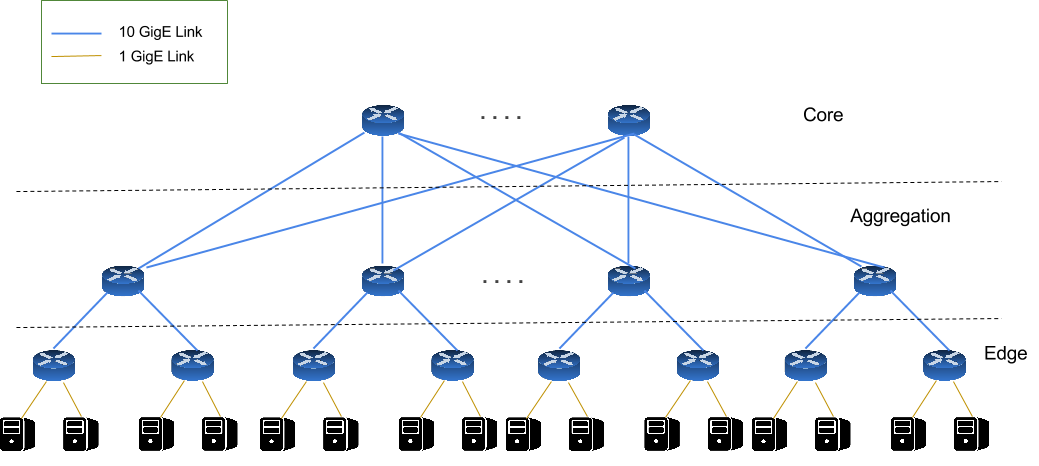
\includegraphics[scale=0.30]{Multi-rootedArch.png}}
	\caption{Common Multi-Rooted Data Centre Architecture with 10 GigE and 1 GigE links.}
	\label{fig:MultiRootedArch}
\end{figure}

At the leaf of a multi-rooted tree topology, there are a number of GigE ports (48-288) with 10 GigE uplinks to one or more switches in the \textit{aggregation layer} \cite{al2008scalable} as illustrated in Figure \ref{fig:MultiRootedArch}. Moving up in the tree hierarchy, switches have 10 GigE ports (32-128), capable of switching significant amounts of traffic between the edges \cite{al2008scalable}. 

Al-Fares \textit{et al.} \cite{al2008scalable} advocate the use of a \textit{fat-tree topology} \cite{leiserson1985fat} for data centre network design and showed that full aggregate bisection bandwidth can be achieved using commodity Ethernet switches of data centre clusters with tens of thousands of hosts. Fat-tree topology aims to alleviate shortcomings in current data centre network design such as

\begin{itemize}

\item over-subscription of links higher up in the topology, where over-subscription is defined by  Al-Fares \textit{et al.} \cite{al2008scalable} to be the ratio of worst-case aggregation bandwidth which can be achieved by the end hosts to the total bisection bandwidth available in the network; where typically, data centre designs are oversubscribed by a ratio of 2.5:1 (400 Mbps) to 8:1 (125 Mbps) with 1 Gb/s commodity Ethernet switches \cite{headquarters2007cisco} and,   

\item the cost of building a network with an over-subscription ratio of 1:1 is quite substantial, with each of the 48-port GigE switch at the edge costing around \$7000, while the 128-port switches at the aggregation and core layer cost around \$700,000 \cite{al2008scalable},
\end{itemize}

by providing backward compatibility to hosts running Ethernet and IP, scaling economically using commodity Ethernet switches for data centre design and providing a scalable interconnection bandwidth enabling any host to communicate with any other host in the network at it’s full local network interface bandwidth \cite{al2008scalable}.

\subsection{Fat-Tree Topology} \label{subsec:Fat-Tree Topology}

\textit{Fat-tree} topology \cite{leiserson1985fat} is a special instance of a \textit{Clos} topology, which was introduced in the 1950s to deliver high levels of bandwidth in telephone networks by interconnecting smaller commodity switches \cite{clos1953study}.  It is organised into \textit{k}-pods, where each pod contains of two layers of \textit{k}/2 switches \cite{al2008scalable}. Each of the \textit{k}/2 hosts in the lower layer are connected directly to each of the \textit{k} port switches in the lower layer of the pod. The remaining \textit{k}/2 ports of each of the switches in the lower layer are connected to \textit{k}/2 ports of the total \textit{k} ports up the hierarchy in the aggregation layer.

The core switches are $\textit{k}/2^2$ in number, with each of the core switch having one port connected to each of the \textit{k} pods . Consecutive ports in the aggregation layer of each pod switch are connected to core switches on \textit{k}/2 strides in such a manner that the ith port of any core switch is connected to pod i. A fat-tree topology built with k-port switches supports $\textit{k}^3/4$ hosts.


\begin{figure}[!ht] 
\centerline{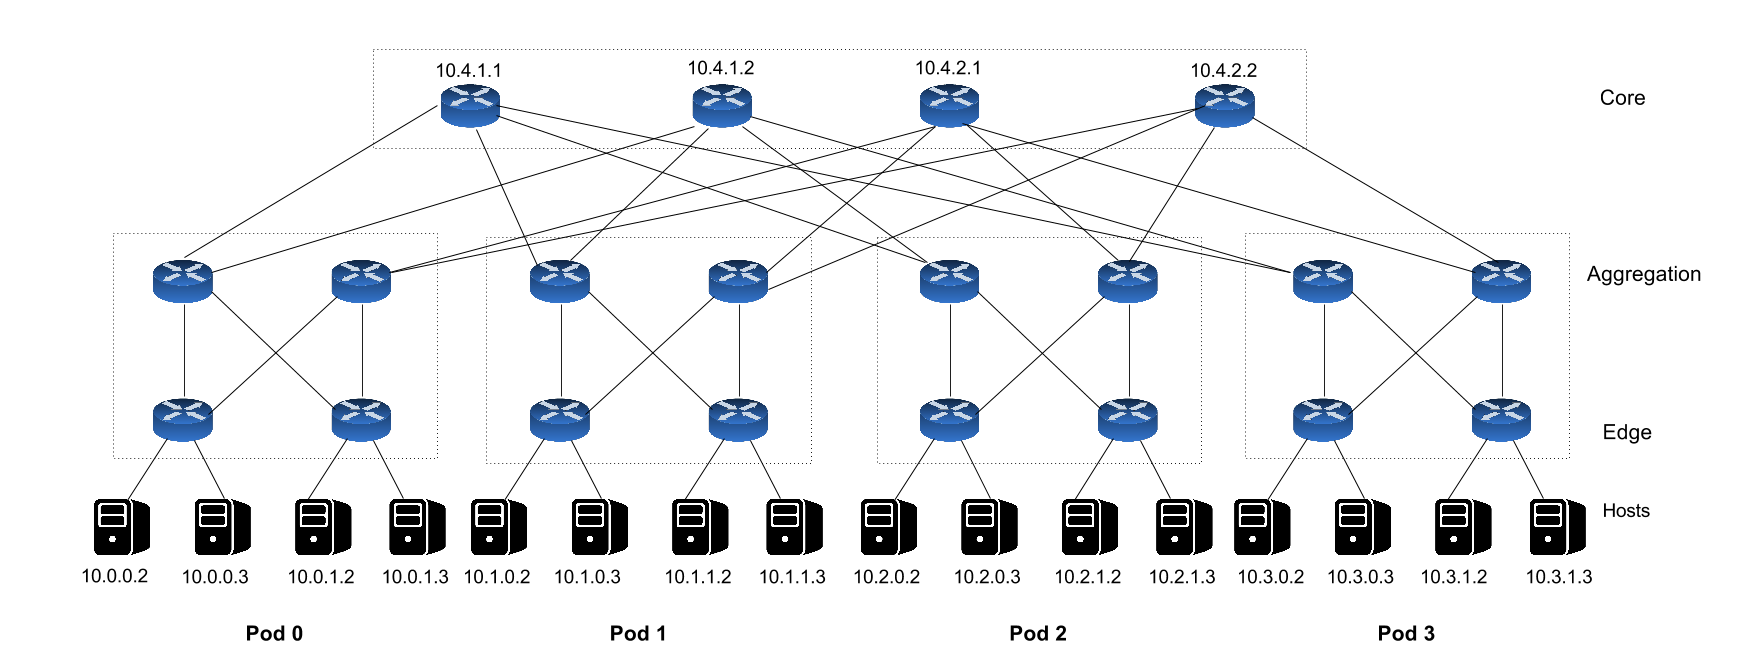
\includegraphics[scale=0.30]{FatTreeTopology.png}}
\caption{Fat-tree topology with 4 pods having 16 hosts in total (k=4).}
\label{fig:FatTreeOverview}
\end{figure}

In this project, we use a fat-tree topology with \textit{k} = 4 for our experiments as described in Chapter \ref{chap:design}. Figure \ref{fig:FatTreeOverview} illustrates a \textit{k}-ary fat-tree topology with \textit{k} = 4, which is the topology we  employ for our experiments. It consists of $\textit{k}^3/4$ i.e. 16 host machines with 4 pods. Hosts connected to the same lower level switch form a subnet; hence, all traffic between two hosts in the same subnet is switched while all the other traffic is routed.

In order to achieve maximum bisection bandwidth in a fat-tree network, outgoing traffic from a pod needs to be spread evenly amongst the core switches. There is a need for the core switches to be able to recognize and provide special behaviour to the traffic classes that need even spreading since  

\begin{itemize}

\item Routing protocols such as OSPF2 \cite{moy1998open} take hop-count as a metric of shortest path, causing switches to concentrate traffic going to a subnet to a single port even though there are $(\textit{k}/2)^2$ paths in the network with the same cost, thereby under utilizing the path diversity in the network and causing severe congestion at these points \cite{al2008scalable}.

\item Extensions to OSPF2 such as OSPF-ECMP \cite{thaler2000multipath} cannot be used on commodity Ethernet switches and require an overwhelmingly large number of prefixes.
 \end{itemize}

To alleviate these shortcomings, Al-Fares \textit{et al.}, devised an addressing scheme that allocates all IP addresses in the network within the private 10.0.0.0/8 block. 

Addressing in a \textit{fat-tree} topology follows the following pattern 

\begin{itemize}
	\item Switches in the pod are allocated IP addresses in the form 10.\textit{pod}.\textit{switch}.1, where \textit{pod} belongs in the range [0, \textit{k}-1], while the \textit{switch} denotes the position of the switch in the pod
	
	\item Core switches are allocated addresses in the form 10.\textit{k}.\textit{j}.\textit{i}, where \textit{j} and \textit{i} denote the co-ordinates of the core switch in the $(\textit{k}/2)^2$ grid 
	
	\item Hosts have addresses of the form 10.\textit{pod}.\textit{switch}.\textit{I D}, where \textit{I D} denotes the host's position in its subnet 
\end{itemize}

This addressing scheme helps in building a two-level routing scheme and scales to 4.2M hosts. The two-level routing scheme enables even spread of traffic across the network \cite{al2008scalable}. Two-level lookup is implemented in hardware using Ternary Contet-Accesible Memory (TCAM).

Due to all these optimizations, Al-Fares \textit{et al.} \cite{al2008scalable} found that in a fat-tree network of 16 hosts, the two-level switches achieve approx. 75\% of the aggregate ideal bisection bandwidth. For their benchmark suite, Al-Fares \textit{et al.} leveraged dynamic flow allocation strategies available in certain routers and found that their flow classifiers performed significantly better than traditional tree topologies which achieve only 28\% of the ideal bandwidth, with the worst-case aggregate bisection bandwidth achieved by the network to be 75\% of the ideal. In light of the results achieved by Al. Fares \textit{et al.}, we choose \textit{fat-tree} topology as the topology of choice for running our simulations described in Chapter \ref{chap:design}.

 
\section{Flow Scheduling in Data Centre Networks} \label{sec:Flow Scheduling in Data Centres}

To take advantage of topologies such as \textit{fat-tree}, described in \ref{subsec:Fat-Tree Topology}, which have multiple paths between the same host-destination pair. In this section, we describe current state-of-the art protocols such as Equal-Cost Multi-Path (ECMP) \cite{hopps2000analysis} and Hedera \cite{al2010hedera} for Multi-Path flow scheduling. These two flow scheduling techniques along with our \textit{proactive} approach are employed in the design of our experiment as described in Chapter \ref{chap:design} and subsequently evaluated against each other in Chapter \ref{chap:eval}.

\subsection{Equal Cost Multi-Path Routing} \label{subsec:ECMP}

Switches that support ECMP are configured with many possible paths for the same host-destination pair. When a packet arrives at a switch, with possible multiple paths to its destination, selected fields of the packet are hashed modulo the total no of paths and the packet is forwarded along the path that corresponds to the result. This results in splitting of the load, maintaining the arrival of packets for the same flow. ECMP is supported by most enterprise switches.

However, ECMP has a lot of limitations, such as it does not take flow bandwidth into account when it makes flow allocation decisions, which can cause bottlenecks at certain links even when the communication pattern is simplistic; this further results in collisions because the static mapping of flows to paths does not take into consideration the current network utilization which overwhelms switch buffers degrading overall performance \cite{al2010hedera}. Moreover, the growth in routing table entries is multiplicative as the number of paths grow causing increase in lookup latency and cost.    

Nonetheless, ECMP implementations support 8-16 multiple paths currently, and it works for topologies such as \textit{fat-tree}, therefore we evaluate it against other approaches, namely Global First-Fit and a proactive approach, for routing of Hadoop traffic as described in Chapter \ref{chap:design} for our current project.

\subsection{Global First-Fit Flow Scheduling} \label{subsec:Hedera}

To alleviate the shortcomings of ECMP described in the previous sub-section, Al-Fares \textit{et al.} \cite{al2010hedera} devised a dynamic flow scheduler called \textit{Hedera}. Hedera is essentially an extension to ECMP; it works similarly to ECMP as described in \ref{subsec:ECMP} for small flows, however when flows exceed a certain threshold rate, \textit{Hedera} dynamically allocates an appropriate path to the flow after doing a demand estimation and installs the path in the appropriate switches. The flow lives only till a certain timeout after which, the flow entries are removed from the path.

The demand estimator converges to the natural flow demand by performing repeated iterations of decreasing the flow capacities at the receivers and increasing it at the sources until the capacities converge. Al-Fares \textit{et al.} devised two algorithms for dynamic flow placement, namely Global First-Fit and Simulated Annealing. In this project, we focus only on Global First-Fit and evaluate it against other approaches of routing Hadoop traffic in a \textit{fat-tree} topology, since it is much simpler to implement than Simulated Annealing.    

When a flow exceeds the threshold rate, Global First-Fit initiates a linear search of all the possible paths that can accommodate the flow and places the flow in the \textit{first} such path that it encounters \cite{al2010hedera}, making it a \textit{greedy}  algorithm. The flows are placed by creating a reservation of the bandwidth capacity along the path and subsequently installing the flow entries in the aggregation and edge switches. Global First-Fit achieves this by maintaining a list of the reserved capacities of all the links in the network and placing flows accordingly.

Al-Fares. \textit{et al.} ran benchmark tests to evaluate the effectiveness of Global First-Fit against ECMP routing in a test bed of 16 hosts arranged in a \textit{fat-tree} topology with OpenFlow \cite{mckeown2008openflow} enabled switches. They also ran tests in a  simulator for measuring the scalability of their routing algorithms. Al-Fares \textit{et al.} \cite{al2010hedera} found that Global First-Fit and Simulated Annealing significantly outperform ECMP for various communication patterns achieving achieving 39\% more of the total bisection bandwidth available in the network, as compared to ECMP.
 